\documentclass[a4paper,11pt]{article}

\usepackage{graphicx}
\usepackage[utf8]{inputenc}
\usepackage{amsmath,amssymb,amsthm,float}
\usepackage[left=20mm,top=20mm]{geometry}

\title{TypeRoids - Typing Accuracy Asteroids - Report}
\author{Marios Igkiempor - 10335752}
\date{May 2019}
 
\begin{document}
\maketitle
 
\section{Description of the Game}
The game is based on typing words(referred to as asteroids) as they fall down the screen.
Typing a word correctly deletes it from the screen.
Typing a word incorrectly still deletes it from the screen, but replaces it with another word.
The new word is shorter with a length equal to the size of the original word minus the number of letters correctly typed, with a minimum length of 3.
Occasionally, magenta power-up words appear on the screen.
These words are either \textit{reset} or \textit{slowdown}.
The reset word moves all the remaining words to the top of the screen, whereas the slowdown word slightly reduces the speed at which words fall down the screen.
The player loses when any word that isn't a power-up word touches the bottom of the screen.
The player wins when all words have been removed from the screen.

As a dependency, the game requires the SDL2 library, on which it relies for the graphics rendering.
SDL was chosen for its cross platform capabilities, allowing the game to be compiled and played on many systems, including all modern computer operating systems.
 
\section{UML Expression of Classes}
\begin{figure}[H]
  \caption{UML Diagram of Classes And Relationships in the Program}
  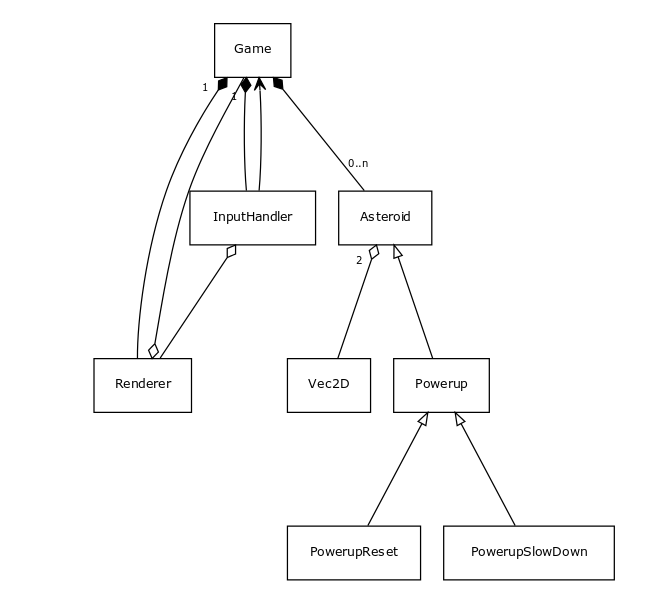
\includegraphics[width=\linewidth]{./uml.png}
\end{figure}

\section{Fulfillment of Requirements}
The program uses C++ object oriented techniques appropriately and correctly.
Examples of inheritance and polymorphism are achieved through the use of the base class \verb|Asteroid| and its subclass \verb|Powerup|. 
\verb|Powerup| is an abstract class which declares a pure virtual method \verb|UsePower()|.
Making this method pure means that an object of type \verb|Powerup| cannot be instanciated directly.
\verb|Powerup| is in turn subclassed into \verb|PowerupSlowDown| and \verb|PowerupReset|, which both define their own implementation of the \verb|UsePower()|.
\verb|PowerupSlowDown| and \verb|PowerupReset| objects are then spawned into the world with a probability defined in the \verb|Constants.h| file.
This hierarchy of classes allows the program to store all the types of ovject in a single \verb|vector| of \verb|Asteroid| pointers, and cast the pointers in the vector to use subclass-specific methods when appropriate.

The simple AI implemented in the game is the one that finds the closest asteroid to the word typed by fuzzy string matching.
It uses the Levenshtein distance between every asteroid and the word typed to determine which asteroid is most similar to the input word.
To optimise the process, it stops calculating Levenshtein distances once a distance of 0 has been found, as it means the word has been typed correctly.
The nearest edit distance, if not 0, is then used as a determinant for the size of the new word to spawn.

\pagebreak
\end{document}
